
\documentclass[letterpaper,twocolumn,10pt]{article}
\usepackage{usenix2019_v3}

% to be able to draw some self-contained figs
\usepackage{tikz}
\usepackage{amsmath}
\usepackage{pgfplots}
\def\code#1{\texttt{#1}}
% inlined bib file
\usepackage{filecontents}

\begin{document}
%-------------------------------------------------------------------------------

%don't want date printed
\date{}

% make title bold and 14 pt font (Latex default is non-bold, 16 pt)
\title{\Large \bf Convolutional Neural Network (CNN) Acceleration with OpenCL}

%for single author (just remove % characters)
\author{
{\rm Robert Geil}\\
University of California, Los Angeles
} % end author

\maketitle

%-------------------------------------------------------------------------------
\begin{abstract}
%-------------------------------------------------------------------------------
Convolutional Neural Networks or \textbf{CNNs} are used by deep learning to
complete many tasks, and especially image recognition. In this lab, we 
accelerated the performance of a CNN using OpenCL, running on an Intel CPU. By
applying techniques in the kernel code such as tiling and vectorization, we
were able to improve performance from the base sequential case of 11 GFlops to
a peak of $\approx 180$  GFlops.
\end{abstract}

%-------------------------------------------------------------------------------
\section{Introduction}
%-------------------------------------------------------------------------------

Convolutional Neural Networks are used in a broad range of fields to perform
automatic categorization of images and data, including image classification,
interpretation of medical results and other applications. As such, the process
of running a CNN would benefit greatly from improvements in performance. In
order to drive some of this performance, we turn to a language called
\textit{OpenCL}. OpenCL, created by an industry group including vendors like
AMD, Intel, NVIDIA, Google, and others, is a programming language used for
heterogeneous computing. With OpenCL, one program can be adapted and run on a
CPU, GPU, FPGA or other computing device, affording flexibility and
portability. Using this language, we will improve and parallelize the
performance of our CNN code. OpenCL also relies on a Host-Kernel system, where
setup code to initialize the system is run on a CPU-based host, while the
Kernels can be more specialized machines like GPUs or FPGAs. As such, our focus
is on writing the Kernel code for performance, rather than host code.

%-------------------------------------------------------------------------------
\section{Machine Specifications}
%-------------------------------------------------------------------------------

As with labs 1 and 2, the machine for which the code was optimized is an Amazon
Web  Services (AWS) \textit{m5.2xlarge} virtual machine. This machine has 4
virtual  CPUs, each of which supports 2 threads via Intel's Hyperthreading
technology. The processor is clocked at 2.5 GHz, and contains 32 Kb L1, 1024 Kb 
L2 and 33792 Kb L3 cache. In addition, the cache line size was 64 bytes. In our
operating region (US N. Virginia), we were supplied with the specific processor
Intel(R) Xeon(R) Platinum 8175M CPU @ 2.50GHz

%-------------------------------------------------------------------------------
\section{Solution Approach}
%-------------------------------------------------------------------------------
To drive the performance improvements desired, the code first needed to be
heavily refactored to permit the use within a kernel, as opposed to on a regular
CPU.

\subsection{Initial Conversion}
As a first step, we attempted to simply port the code from the sequential
version into the kernel. However, this caused an issue where an exception of
\textbf{CL\_OUT\_OF\_RESOURCES} was raised. This was determined to be due to
the fact that the \code{float C[]} matrix was too large for the memory of each
kernel. Therefore we needed to break up the matrix. The initial attempts to
reduce down to a single thread per 4 values in C (which are pooled to the
output) proved to be too fine-grained parallelism, providing a performance of
\textbf{approximately 18 GFlops}

\subsection{Coarser-grained Parallelism}
To improve on our performance by reducing the number of threads, we pooled so
that each thread handled two rows of length 224, writing then to one row of
the output. This reduced the number of threads by a factor of 56, and ended up
improving the performance to \textbf{approx 30 GFlops}.

\subsection{OpenCL Vectorization}
In addition to the typical C data types, OpenCL provides vectorized versions,
such as \code{float4}, \code{float16}, \code{int16} and others. Since modern
processors and GPUs have extensions built in allowing for operations on larger
sets of bits, using these vector data types allows, for example, 16 floats to
be added in the time that one would typically take with instruction-level
parallelism. We took advantage of this in our code, rewriting our local array
to store \code{float16} values, rather than regular floats. This meant that
the number of raw computations we needed to complete was reduced by a factor
of 16, although conversion overhead and other limitations reduced this benefit.
By this conversion, we were able to push our performance up to 
\textbf{approximately 130 GFlops}. However, this is still below the range of
an A, meaning that more optimization was required.

\subsection{Loop Tiling}
In order to improve memory access and cache hit rates, we turned to loop
tiling for the final optimization. Within the convolution step, we tiled the
\code{j} and \code{w} loops, and reordered the loops such that the inner
loop of \code{w} was the innermost loop. This last step improved our
performance to \textbf{approx 150 GFlops}.

\subsection{Memory Localization}
One minor modification which gained an additional 30 GFlops was moving from
local to private memory. This change improved performance, as private memory
doesn't need to be shared across threads in the same work group. Adding this
optimization gave a final performance of \textbf{approximately 180 GFlops}.

%-------------------------------------------------------------------------------
\section{Results}
%-------------------------------------------------------------------------------
\subsection{Performance}
As described above, applying our optimizations in coarse-grained parallelism,
vectorization, loop tiling and memory localization yielded a final performance
of $\approx 180$ GFlops. This was with the threads split so that there were 256
threads in global group 0, and 112 in group 1, giving an arrangement of
(256, 0). By splitting this way, we reduced the number of loops that each
individual had to go through.
\subsection{Thread Number Impact}
Because of the way the kernel code was written, global group 0 can be any value
from 1 to 256 for properly splitting up the program and writing the correct
output, while the second group must be 112, as that is value of
\code{kOutImSize}. This was slightly modified to produce the graph as see in
figure~\ref{fig:threads}. In the figure, there is a rapid increase in the 
performance as threads increase from 1 to 8, with an interesting lack of major
jump from 2 to 4 threads. However, we see that upon reaching 8 threads, there
is little change in performance, as any number beyond that is being virtualized
given that there are only 4 physical cores and 8 threads. Results of the
sequential and OpenCL versions can be seen in figure~\ref{table:perf}.
\begin{figure}
  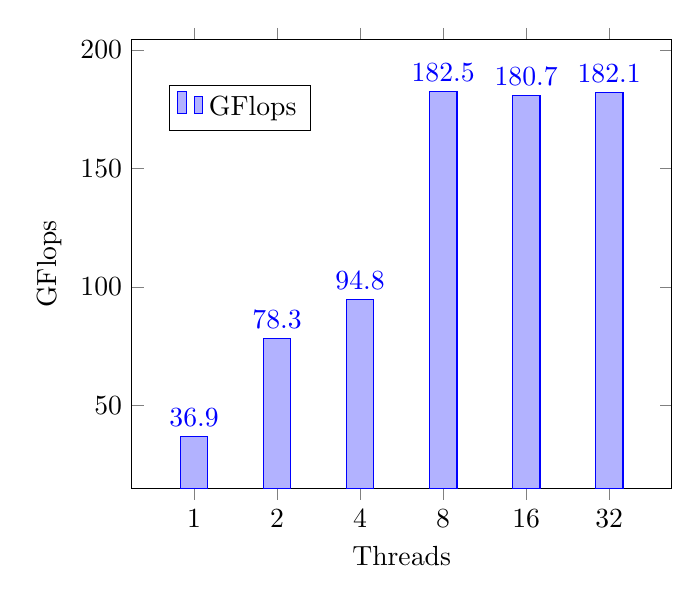
\begin{tikzpicture}
    \begin{axis}[
        ybar,
        enlargelimits=0.15,
        legend style={at={(0.2,.9)},
          anchor=north,legend columns=-1},
        ylabel={GFlops},
        xlabel={Threads},
        symbolic x coords={1,2,4,8,16,32},
        xtick=data,
        nodes near coords,
        nodes near coords align={vertical},
        ]
        \addplot coordinates {(1,36.9) (2,78.3) (4,94.8) (8,182.5) (16,180.7) (32, 182.1)};
    \legend{GFlops}
    \end{axis}
    \end{tikzpicture}
    \caption{\label{fig:threads} Performance of the CNN with various numbers of
    threads}
\end{figure}
\begin{figure}
  \begin{center}
    \begin{tabular}{|c|c|c|}
      \hline
      Type & Global Workgroup & Performance\\
      \hline
      Sequential & N/A & 11.5 GFlops \\
      OpenCL & (1, 1) & 36.9 GFlops \\
      OpenCL & (2, 1) & 78.3 GFlops \\
      OpenCL & (4, 1) & 94.8 GFlops \\
      OpenCL & (8, 1) & 182.5 GFlops \\
      OpenCL & (256, 112) & 182.8 GFlops \\
      \hline 
    \end{tabular}
  \end{center}
  \caption{\label{table:perf} Performance of the Kernel CNN compared to the 
  Sequential Version}
\end{figure}
%-------------------------------------------------------------------------------
\subsection{Challenges}
This project ended up being more time consuming and difficult than previously
expected. One of the first major challenges I faced was the issue described in
the introduction, of the \textbf{CL\_OUT\_OF\_RESOURCES} error. While I was
eventually able to find what was causing the error, it took quite a while, and
was complicated by the lazy evaluation that OpenCL does, meaning that if the
\code{C} array was never read from, this error wouldn't occur. This threw me
off the trail of tracking this issue. Another problem I faced was simply getting
used to the vector data types, and finding out what operations meant in terms
of the vector rather than individual components. For example, that multiplying
two vectors resulted in a dot-product. Finaly, it was challenging to understand
the basis of the CNN and what it was attempting to do, which complicated further
the job of optimizing it.
%-------------------------------------------------------------------------------
\end{document}
%%%%%%%%%%%%%%%%%%%%%%%%%%%%%%%%%%%%%%%%%%%%%%%%%%%%%%%%%%%%%%%%%%%%%%%%%%%%%%%%